\subsubsection{概要}
むぎまるチームは1章の通り、「自己位置推定の破綻を修復できる自己位置推定器の開発」
を目標としてシステムを構成した。
そのため自己位置推定には、LiDARベースのMonte Carlo localization(MCL)と、
膨張リセット\cite{ueda2004iros}により破綻を修復する機能が
実装されたemcl2\_ros2パッケージ\cite{emcl2_ros2}を使用した。
次項では詳細のシステム構成を説明する。
\subsubsection{システム構成}
むぎまるチームのシステム構成について説明する。
ロボットに搭載した計算機、センサ、アクチュエータの接続の関係及び
計算機で実行するROS 2ノードの概要を表したものを
図\ref{fig:mugimaru_system}に示す。

Raspberry Piには、IMUとエンコーダ、車輪駆動用の
モータを接続した。
実行するノードとしては、IMU用のROS 2ドライバーノード(rt\_usb\_9axisimu\_driver)と、
オドメトリの出力とモータの制御を実施するノード(raspimouse)がある。
後者のノードでは、エンコーダの値と
前者のノードで配信されたIMUの情報からロボットのオドメトリを計算し、
トピックとして配信する。
モータの制御は、外部のノードからトピックとして受信した
ロボットの速度指令をもとに実行する。

PCには、3D LiDARとRaspberry Piを接続した。
実行するノードとしては、3D LiDAR用のノードが2つ、
ロボットの自己位置推定とナビゲーションを実行するノードがある。
3D LiDAR用のノードとしては、Livox用のROS 2ドライバーノード(livox\_lidar\_publisher)と、
3D LiDARからの3次元点群を2次元に圧縮し、
トピックとして配信するノード(pointcloud\_to\_laserscan)がある。
自己位置推定には、前項のとおりemcl2\_ros2パッケージ\cite{emcl2_ros2}を使用した。
図中には、ノード名として「emcl2」と表している。
このパッケージでは、走行する環境の地図と
オドメトリ、2次元のLiDARデータを使用して、
ロボットの推定位置をtfの形式で出力する。
この地図の作成には、slam\_toolboxパッケージ\cite{slam_toolbox}を使用した。
ナビゲーションには、navigation2パッケージ\cite{nav2}を使用した。
図中には、このパッケージに内包されるノードをまとめて「navigation2」と表している。

\begin{figure}[h]
  \begin{center}
    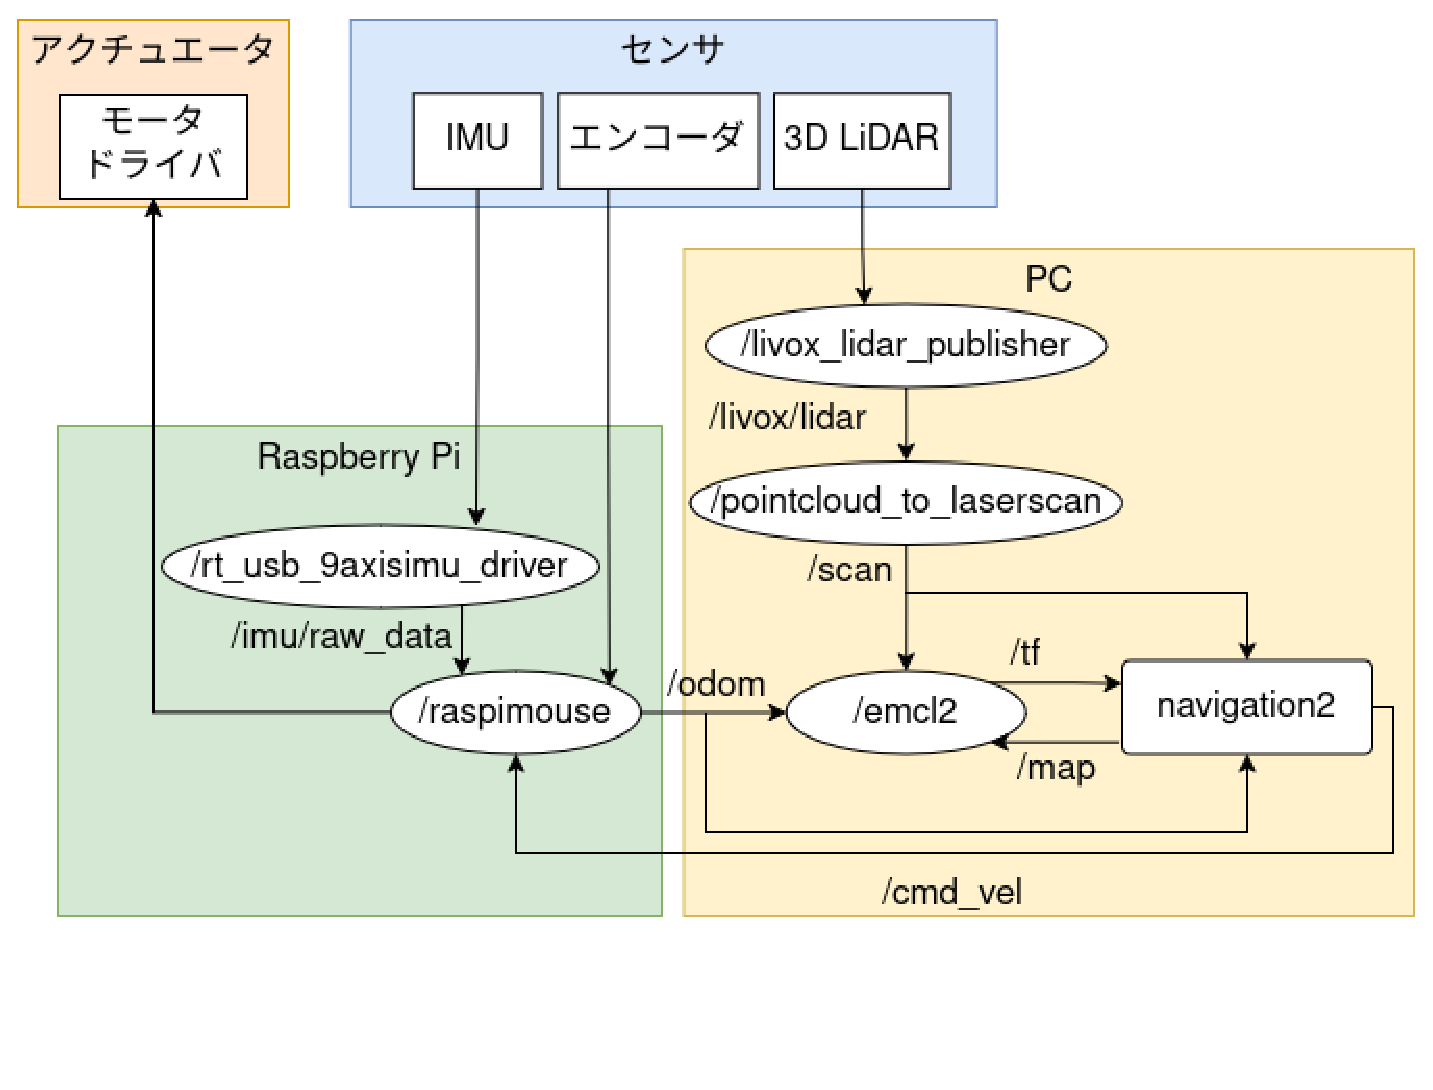
\includegraphics[width=1.0\linewidth]{figs/mugimaru_system_2024.eps}
    \caption{むぎまるチームのシステム構成}
    \label{fig:mugimaru_system}
  \end{center}
\end{figure}

